\documentclass{article}
\usepackage{setspace}
\usepackage{geometry}
\usepackage[utf8]{inputenc}
\usepackage{amsmath,amsthm,amssymb,bm}
\usepackage{mathtools}

\geometry{letterpaper, portrait, margin=1in}
\setstretch{1.5}
\title{Homework 12}
%\date{1-18-2020}
\author{Runmin Lu}

\begin{document}
	\maketitle
	%\newpage
	
	\section*{1}
	\subsection*{(a)}
		identity:
		\begin{align*}
			\frac{\delta e}{\delta W_1} &\approx
			\begin{pmatrix}
				-0.01938197 & -0.01938197\\
				-0.01938197 & -0.01938197\\
				-0.03876394 & -0.03876394       			
			\end{pmatrix}\\
			\frac{\delta e}{\delta W_2} &\approx
			\begin{pmatrix}
				-0.18460146\\
				-0.14059139\\
				-0.14059139
			\end{pmatrix}
		\end{align*}
		tanh:
		\begin{align*}
			\frac{\delta e}{\delta W_1} &\approx
			\begin{pmatrix}
				-0.01594156 & -0.01594156\\
				-0.01594156 & -0.01594156\\
				-0.03188311 & -0.03188311
       		\end{pmatrix}\\
			\frac{\delta e}{\delta W_2} &\approx
			\begin{pmatrix}
				-0.15183362\\
				-0.1156356\\
				-0.1156356
			\end{pmatrix}
		\end{align*}
	\subsection*{(b)}
		identity:
		\begin{align*}
			\frac{\delta e}{\delta W_1} &\approx
			\begin{pmatrix}
				-0.01938022 & -0.01938022\\
				-0.01938022 & -0.01938022\\
				-0.03875693 & -0.03875693
			\end{pmatrix}\\
			\frac{\delta e}{\delta W_2} &\approx
			\begin{pmatrix}
				-0.18457646\\
				-0.14057689\\
				-0.14057689
			\end{pmatrix}
		\end{align*}
		tanh:
		\begin{align*}
			\frac{\delta e}{\delta W_1} &\approx
			\begin{pmatrix}
				-0.01594012 & -0.01594012\\
				-0.01594012 & -0.01594012\\
				-0.03187736 & -0.03187736
			\end{pmatrix}\\
			\frac{\delta e}{\delta W_2} &\approx
			\begin{pmatrix}
				-0.15181331\\
				-0.11562382\\
				-0.11562382
			\end{pmatrix}
		\end{align*}
		
	\section*{2}
	\subsection*{(a)}
		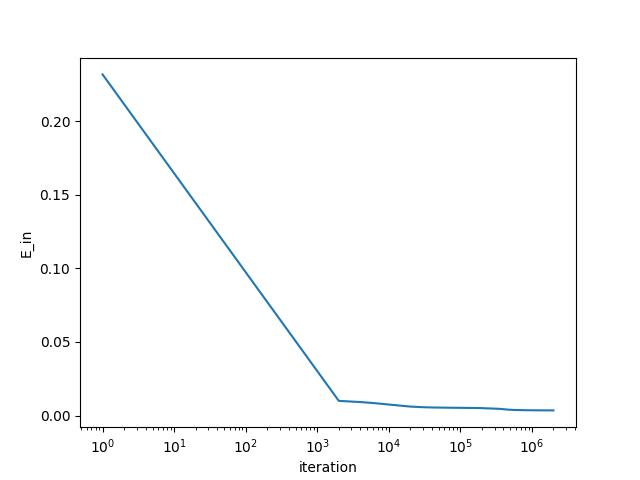
\includegraphics[scale=0.8]{2a1}\\
		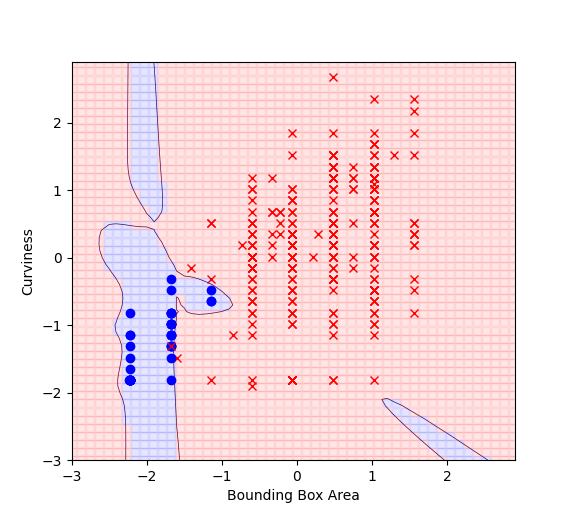
\includegraphics[scale=0.8]{2a2}
		
	\subsection*{(b)}
		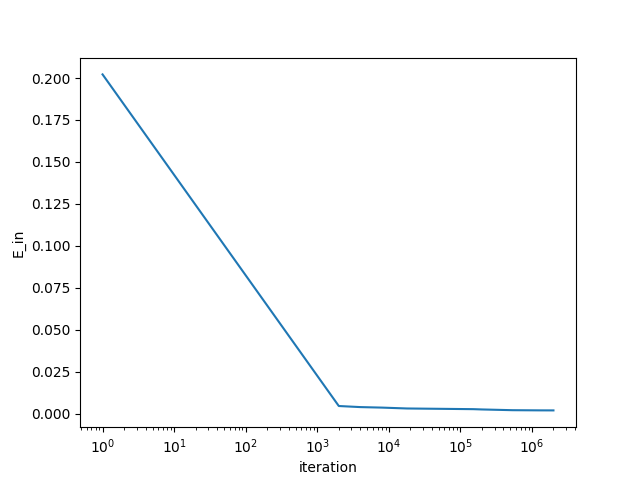
\includegraphics[scale=0.8]{2b1}\\
		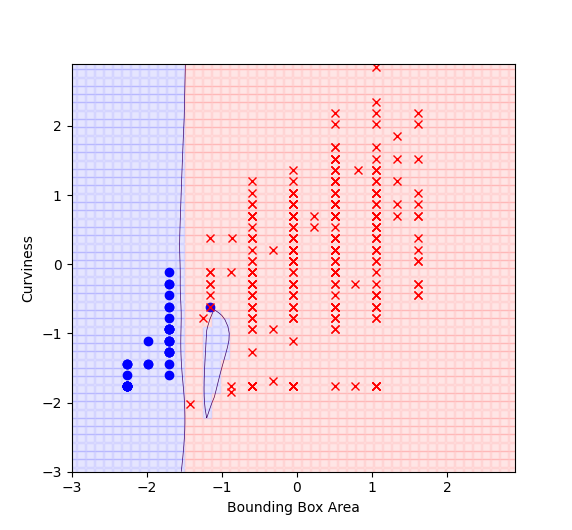
\includegraphics[scale=0.8]{2b2}
		
	\subsection*{(c)}
		Since $E_\text{in}$ reduces much more slowly after about the 2000th iteration, I inferred that iterations after that will overfit. Therefore, from a list of $100x$ for integer $x \in [1, 20]$, the optimal number of iterations is 100 with $E_\text{test} \approx 0.0139$.\\
		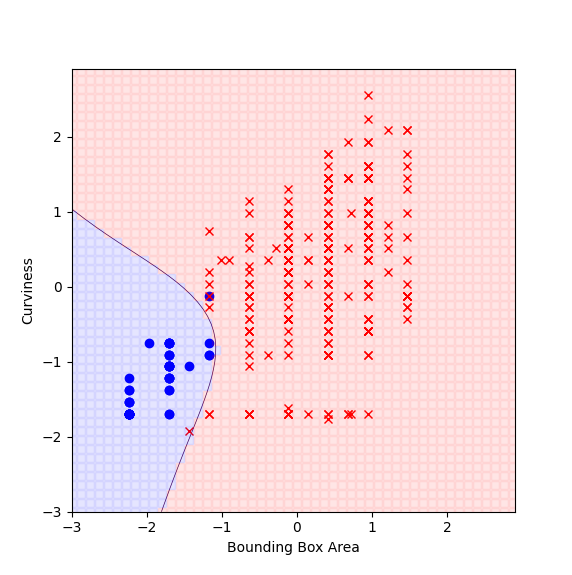
\includegraphics[scale=0.8]{2c}
		
	\section*{3}
	\subsection*{(a)}
		Let the optimal hyperplane be $ax + by + c = 0$. Then the distance to $\mathbf x_1$ is $\frac{|a + c|}{\sqrt{a^2 + b^2}}$ and the distance to $\mathbf x_2$ is $\frac{|-a + c|}{\sqrt{a^2 + b^2}}$. To maximize those values, we want to minimize the denominator, so we set $b = 0$ and the hyperplane becomes a vertical line.\\
		Since $\mathbf x_1$ and $\mathbf x_2$ must be on different sides of the line, to maximize the minimum of the distances, we set $\frac ca = 0$. Therefore, $c = 0$ and $a \neq 0$. WLOG let $a = 1$ and the corresponding line becomes $x_1 = 0$,  which is in fact their perpendicular bisector.\\
		To make the right side +1, we have $\mathbf w = (1, 0), b = 0$.
	\subsection*{(b)}
		$\mathbf z_1 = (1, 0), \mathbf z_2 = (-1, 0)$. Since the coordinates are the same, the perpendicular bisector is the same: $z_1 = 0$.\\
		Optimal hyperplane: $\mathbf w = (1, 0), b = 0$.
		
	\subsection*{(c)}
		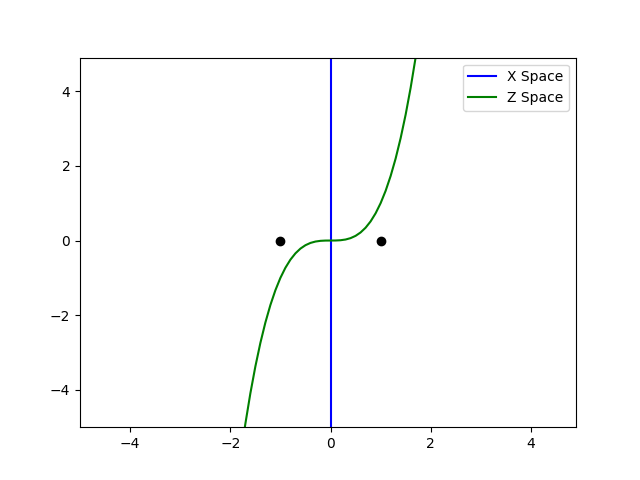
\includegraphics[scale=0.8]{3c.png}
		
	\subsection*{(d)}
		\begin{align*}
			K(\mathbf x, \mathbf y) &= \mathbf z(\mathbf x) \cdot \mathbf z(\mathbf y)\\
			&=
			\begin{pmatrix}
				x_1^3 - x_2\\
				x_1x_2
			\end{pmatrix}
			\cdot
			\begin{pmatrix}
				y_1^3 - y_2\\
				y_1y_2
			\end{pmatrix}\\
			&= \boxed{(x_1^3 - x_2)(y_1^3 - y_2) + x_1x_2y_1y_2}
		\end{align*}
		
	\subsection*{(e)}
		\begin{align*}
			g(\mathbf x) &= \text{sign}(\mathbf w \cdot \mathbf z(\mathbf x) + b)\\
			\mathbf w &= \alpha_1y_1\mathbf z(\mathbf x_1) + \alpha_2y_2\mathbf z(\mathbf x_2)\\
			(1, 0) &= \alpha_1(1, 0) - \alpha_2(-1, 0)\\
			1 &= \alpha_1 + \alpha_2\\
			\text{Dual Constraint: } 0 &= \alpha_1y_1 + \alpha_2y_2\\
			&= \alpha_1 - \alpha_2\\
			\alpha_1 &= \frac12\\
			\alpha_2 &= \frac12\\
			g(\mathbf x) &= \text{sign}((\frac12\mathbf z(\mathbf x_1) - \frac12\mathbf z(\mathbf x_2)) \cdot \mathbf z(\mathbf x) + b)\\
			&= \boxed{\text{sign}(\frac12 K(\mathbf x_1, \mathbf x) - \frac12 K(\mathbf x_2, \mathbf x))}
		\end{align*}
	
	\section*{4}
	\subsection*{(a)}
		Small $C = 0.0001$:\\
		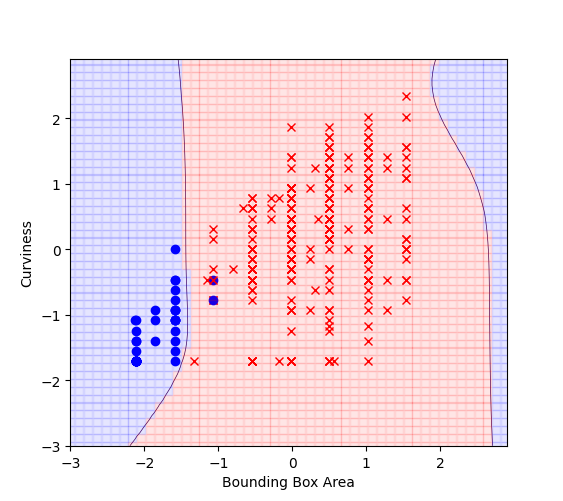
\includegraphics[scale=0.7]{4a1}\\
		Large $C = 1000$:\\
		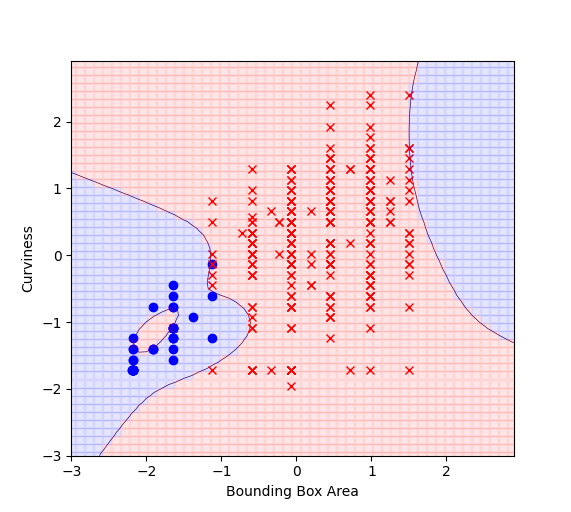
\includegraphics[scale=0.7]{4a2}
		
	\subsection*{(b)}
		Since the quadratic program has constraints: $\forall i: 0 \leq \alpha_i \leq C$, as $C$ gets smaller, each $\alpha_i$ is more constrained and the feasible regions becomes smaller, which corresponds to more regularization.\\
		It can be seen from the plots that the decision boundary resulted from large $C$ is much more curvy and complex. Although both models overfit with the right blue region, the one with large $C$ has a really unnecessary red hole on the lower left.
		
	\subsection*{(c)}
		From a list of $2^x$ for integer $x \in [-10,10$], the optimal $C = 1$ with $E_\text{test} \approx 0.0180$\\
		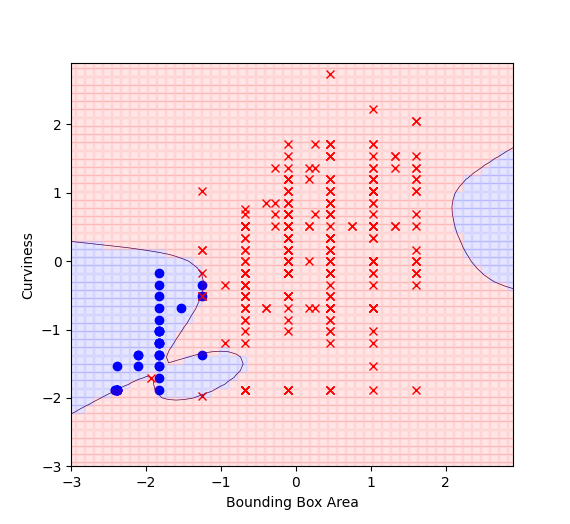
\includegraphics[scale=0.7]{4c}
		
	\section*{5}
		\begin{tabular}{c|c}
			Model & $E_\text{test}$\\
			\hline
			Linear & 0.0111\\
			k-NN & 0.0127\\
			RBF & 0.0139\\
			Neural Network & 0.0139\\
			SVM & 0.0180
		\end{tabular}\\\\
		If we compare models only based on $E_\text{test}$, then we would pick the linear model as the best one. However, that shouldn't be the only factor, especially when these $E_\text{test}$'s are close because they can be above or below $E_\text{out}$ by a factor of $\frac1{\sqrt K}$ where $K$ is the number of test points. If we examine more, we can see that the decision boundaries of k-NN (shown below) and neural network are much less complex than other models (shown below), which all have some blue regions on the right. Therefore, k-NN and neural network overfit the least and are two of the best models for this problem.\\
		In addition, if we think intuitively, SVM is generally not a good model for inseparable data, which defeats the whole purpose of SVM (maximum margin). This explains why it has the largest $E_\text{test}$ among all the models.\\\\
		k-NN:\\
		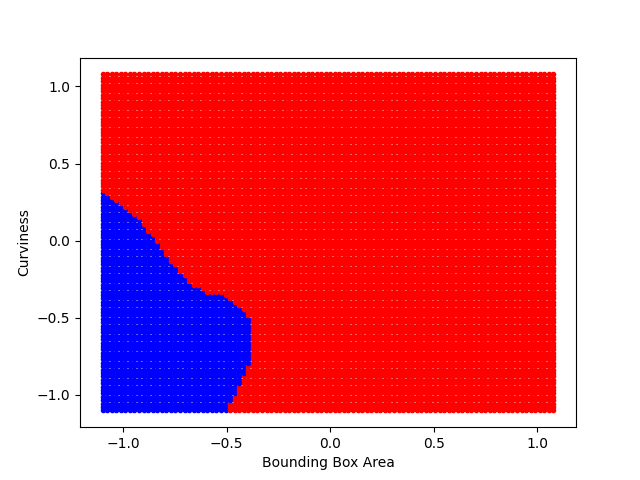
\includegraphics[scale=0.8]{../hw11/1b}\\
		RBF:\\
		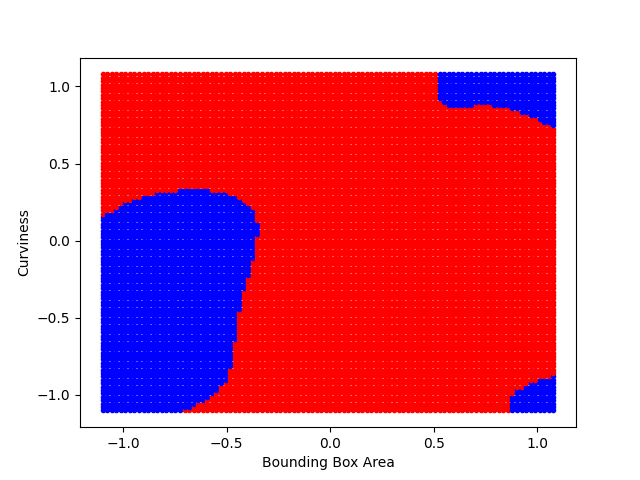
\includegraphics[scale=0.8]{../hw11/2b}\\\\\\\\
		Linear:\\
		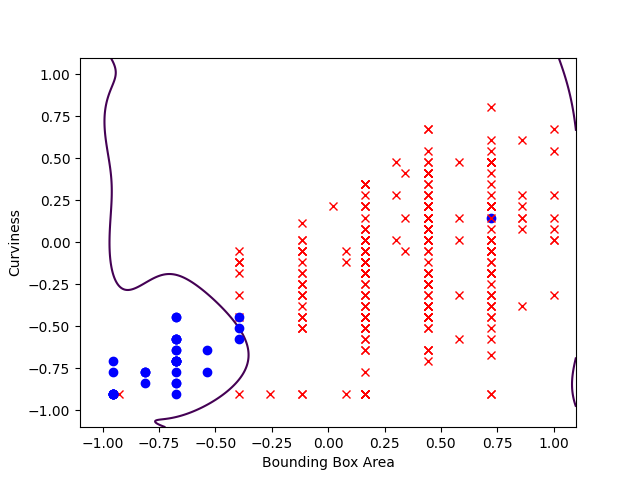
\includegraphics[scale=0.8]{../hw09/3}
\end{document}